\usepackage{amsthm}
\usepackage{booktabs}
\usepackage[T1]{fontenc}
\usepackage[margin=1in]{geometry}
\usepackage{mathtools}
\usepackage{microtype}
\usepackage{minted}
\usepackage{natbib}
\usepackage{newpxmath}
\usepackage{newpxtext}
\usepackage{rgalg}
\usepackage{thmtools}
\usepackage{tikz}
\usepackage{xcolor}

\usepackage{hyperref}

\usepgflibrary{arrows}
\usetikzlibrary{matrix}

\definecolor{darkblue}{rgb}{0,0,0.4}
\definecolor{darkgreen}{rgb}{0,0.4,0}
\hypersetup{colorlinks,linkcolor=darkblue,citecolor=darkblue,urlcolor=darkblue}

\usemintedstyle{tango}
\newminted{c}{linenos}
\newminted{java}{linenos}

\renewcommand*\.[1]{{\sf#1}}

\newcommand*\lecture[1]{
  \centerline{
  \framebox[1.05\textwidth]{\vbox{
    \hbox to\textwidth{{\bf CO527: Operating Systems}\hfil Spring 2017}
    \vspace{3ex}
    \hbox to\textwidth{\hfil\Large\bf#1\hfil}
    \vspace{3ex}
    \hbox to\textwidth{\it Radu Grigore\hfil}
  }}}
  \vspace{5ex}\par
}

\newcommand*\asgn\coloneqq
\newcommand*\df\emph
\newcommand*\todo[1]{\marginpar{\raggedright\tiny\color{darkgreen}TODO: #1\par}}
\newcommand*\defeq\coloneqq

\declaretheorem{theorem}
\declaretheorem[sibling=theorem]{lemma}

\title{Operating Systems Concepts}
\author{Radu Grigore}

\begin{document}
\lecture{Schedulers}

\section*{Threads and Schedules}

\noindent
A \df{scheduler} is an operating system component
  that decides which thread runs on which processing unit.
In this note, from now on, we say `core' rather than the longer `processing unit'.
As an example,
  consider a situation in which we have $2$~cores,
  and the following requests:
\begin{enumerate}
\item at time~$1$, thread~A starts to run;
  it will finish after it gets to run for $3$~time units
\item also at time~$1$, thread~B start to run;
  it will finish after it gets to run for $2$~time units
\item at time~$2$, thread~C starts to run;
  it will finish after it gets to run for $4$~time units
\item at time~$3$, thread~D starts to run;
  it will finish after it gets to run for $1$~time unit
\item and finally, at time~$6$, thread~E starts to run;
  it will finish after it gets to run for $1$~time unit
\end{enumerate}
Given such a list of requests,
  a scheduler must find a \df{schedule}:
  for each unit of time, which thread executes on which core.
For example,
  the figure below illustrates three possible schedules for the requests above:
\begin{center}
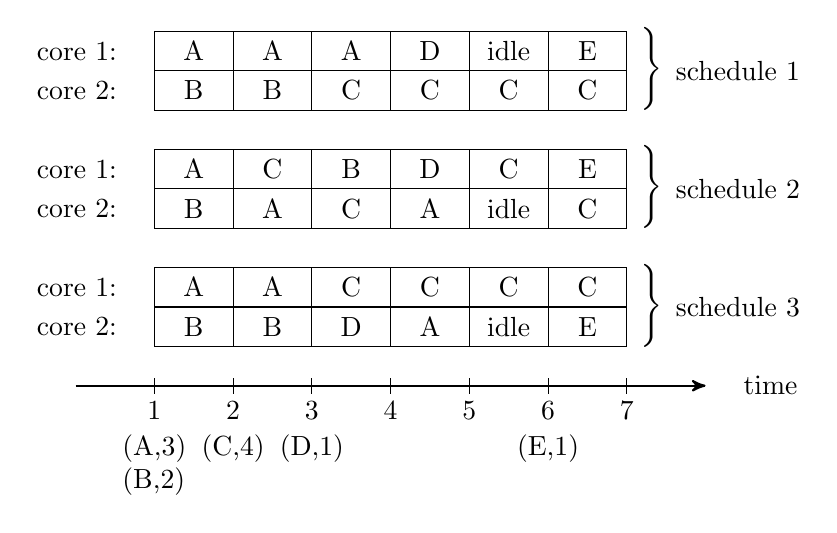
\begin{tikzpicture}[yscale=.5]
\newcommand\core[3]{
  \draw (0,#2) \foreach \x in {#3} {++(1,0) rectangle node{\x} +(1,1)};
  \node[anchor=east] at (1,#2+0.5) {\hbox{core #1:\quad}};
}
\newcommand\lbl[2] {
  \node[left delimiter=\},xshift=5mm,anchor=west,minimum height=1cm] at (7,#1) {schedule #2};
}
\tikzset{arr/.style={->,>=stealth'}}
\draw[thick,arr] (0,0) -- (8,0) node[right=10pt] {time};
\core{1}{8}{A,A,A,D,idle,E};
\core{2}{7}{B,B,C,C,C,C}; \lbl{8}{1};
\core{1}{5}{A,C,B,D,C,E};
\core{2}{4}{B,A,C,A,idle,C}; \lbl{5}{2};
\core{1}{2}{A,A,C,C,C,C};
\core{2}{1}{B,B,D,A,idle,E}; \lbl{2}{3};

\foreach \x in {1,...,7} {
  \draw (\x,-0.2) -- (\x,0.2);
  \node[below=.5ex] at (\x,0) {\x};
}
\node[align=left,anchor=north] at (1,-1) {(A,3)\\(B,2)};
\node[align=left,anchor=north] at (2,-1) {(C,4)};
\node[align=left,anchor=north] at (3,-1) {(D,1)};
\node[align=left,anchor=north] at (6,-1) {(E,1)};
\end{tikzpicture}
\end{center}
Below the time axis, we have labels of the form $({\it thread},{\it duration})$,
  which correspond to the events listed above.
The time units are arbitrary:
  for an operating system like Linux, the time unit is $\sim10$~ms.
Let's look at the label $(D,1)$, which is under time~$3$.
It says that D requires one unit of time.
Indeed, in schedule~1, thread~D runs on core~1 in the time interval $(4,5)$;
  in schedule~1, it runs on core~1 in the time interval $(4,5)$;
  and in schedule~2, it runs on core~2 in the time interval $(3,4)$.
Notice that all intervals are after time~$3$ when the request arrived.

\subsection*{Properties of Schedules}

Schedules have several characteristics,
  such as response time, (core) utilisation, and context switching.

The \df{response time} of one thread in a given schedule
  is the time passed since the thread requests to start until it thread finishes.
The \df{total response time} of a schedule
  is the sum of the response time of all the threads in that schedule.
The \df{delay} of one thread in a given schedule
  is the difference between the response time and the duration that thread runs.
The \df{total delay} of a schedule
  is the sum of the delays of all the threads in that schedule.
For example, in the example above,
  the request times, the finish times, the response times, and the delays
  are as follows:
\begin{center}
\begin{tabular}{@{}lrrrrrrrrrrr@{}}
\toprule
  & & &
  \multicolumn{3}{c}{Finish} &
  \multicolumn{3}{c}{Response} &
  \multicolumn{3}{c}{Delay} 
  \\
    \cmidrule(lr){4-6} \cmidrule(lr){7-9} \cmidrule(l){10-12}
Thread  & Request & Runtime & 1 & 2 & 3 & 1 & 2 & 3 & 1 & 2 & 3 \\
\midrule
A & 1 & 3 & 4 & 4 & 4 & 3 & 3 & 3 & 0 & 0 & 0 \\
B & 1 & 2 & 3 & 4 & 3 & 2 & 3 & 2 & 0 & 1 & 0 \\
C & 2 & 4 & 7 & 7 & 7 & 5 & 5 & 5 & 1 & 1 & 1 \\
D & 3 & 1 & 5 & 5 & 4 & 2 & 2 & 1 & 1 & 1 & 0 \\
E & 6 & 1 & 7 & 7 & 7 & 1 & 1 & 1 & 0 & 0 & 0 \\
{\bf Total} & & & & & & \bf 13 & \bf 14 & \bf 12 & \bf 2 & \bf 3 & \bf 1 \\
\bottomrule
\end{tabular}
\end{center}
We see that schedule~3 has the smallest total response time
  and the smallest total delay.
So, schedule~3 is the best with respect to response times.

Another way to evaluate schedules is to look at core utilisation.
The \df{utilisation} of a core
  is the number of time steps it was active (non-idle)
  divided by the total number of steps.
The \df{total utilisation} of a computer is the sum of utilisations over all cores.
(Sometimes the term `load' is used instead of `utilisation'.)
In our example, the total utilisation is $1.8(3)$ for all three schedules.
In general, higher utilisation indicates that less time is wasted,
  with cores being idle and not doing work.

Finally, another way to evaluate schedules is to count context switches.
A \df{context switch} is a transition from one thread to another, on one core,
  ignoring idle times.
So, for example, core~1 in schedule~1 has one context switch ${\rm A}\to{\rm D}$,
  and one context switch ${\rm D}\to{\rm E}$.
In total, schedules 1, 2, 3 have, respectively, 3, 9, and 4 context switches.
We care about context switches because they imply delays:
  for example, the caches local to one core are not that helpful
  after a context switch.
So, schedule~1 is the best with respect to the number of context switches.

\subsection*{Real Time}

As we saw, there are several measures we can use to gauge how good schedules are.
We can also combine several measures.
For example,
  we could say that schedule~$X$ is better than schedule~$Y$
  when the total delay of~$X$ is smaller than the total delay of~$Y$,
    or the total delays are equal but $X$ has a smaller maximum delay per thread.%
\footnote{
  More briefly, we'd say we use the lexicographic order on
  $(\text{total delay}, \text{maximum delay})$.
}
\df{Real time applications} are those which strongly prefer schedules
  with small maximum delays per thread.
\df{Hard real time applications} have a deadline:
  all schedules with a maximum delay exceeding the deadline just as bad ---
  they are unusable.
That is, if two schedules both exceed the deadline,
  then it makes no sense to say which of them is better.
\df{Soft real time applications} are real time applications that are not hard.%
\footnote{
  One could still use a deadline with soft real time applications.
  In that case, schedules would use the lexicographic order on
    (count of deadline misses, maximum deadline, something else).
}

Real time applications usually produce periodic requests for the scheduler.
For example,
  Skype might have a thread that every $50$~ms compresses the audio data
  captured in the previous $50$~ms.
This leads us to an interesting problem.
Suppose that compressing $50$~ms of audio data takes $T$~ms.
Can we find a schedule?
Well, it depends on~$T$, but also on the number of cores~$N$.
An easy way to tell is as follows:
  It is possible if and only if the total utilisation is~$\le N$.
But, how total utilisation is a property of a schedule:
  How can we compute it if we don't even know whether a schedule exists?
Since the requests are periodic,
  it is reasonable to expect that if a schedule exists then a periodic schedule exists. \todo{prove}
Now, if we look at a long enough time of~$D$~ms,
  for any schedule,
    the number of requests will be $D/50$
    and the nonidle time will be $DT/50\pm NT$.
The error can't be bigger than $NT$. (Exercise: Why?)
And, of course, the time available to each core is~$D$.
Thus, total utilisation is
\begin{align*}
\frac{\frac{DT}{50} \pm NT}{D}
  = \frac{T}{50} \pm \frac{NT}{D}
\end{align*}
Since this is true for any~$D$ (we chose it arbitrarily),
  we just let $D\to\infty$ to make the error arbitrarily small.
Finally, we get that the total utilisation is $T/50$,
  as we'd have guessed immediately if wouldn't have wanted to check more carefully.
And here is the simple criterion:
  Total utilisation cannot exceed the number of cores.
If it does, we say that the requests are \df{not schedulable}.



\section*{Schedulers}

Now let us look at a few scheduling algorithms.

\subsection*{FIFO Scheduler}

A FIFO scheduler maintains a queue of threads waiting to run.
When a new request arrives,
  it is enqueued,
  unless there is an idle processor where the thread can begin execution immediately.
When a thread finishes and its core becomes available,
  the next thread from the queue is given the available core.
Threads always run to completion.

As an example, schedule~1 from above is produced by a FIFO scheduler.
You can find a FIFO scheduler simulator in the accompanying \.{FifoScheduler.java}.


\subsection*{Round Robin Scheduler${}^\ast$}
\todo{Make it non-optional?}

A round robin scheduler is similar to a FIFO scheduler.
The main difference is that threads do not run to completion.
Instead they run for just one time step, and then are moved back in the queue.

The accompanying \.{RoundRobingScheduler.java} contains a simulator.
Let us look at its most important parts.
The simulator reads in a list of requests like the following:
\begin{verbatim}
2
1 A 3
1 B 2
2 C 4
3 D 1
6 E 1
\end{verbatim}
This corresponds to our previous example.
The first line gives the number of available cores.
The second line says that, at time~1, thread~A is created,
  and thread A will finish after it will run for 3~time steps.
The third and following lines have the same format as the second line.
The number of cores is stored in integer~\.{n};
  the rest is stored in a \.{Deque$\langle$Task$\rangle$} called \.{input}.
The fact that we parse all the input before doing any work
  and the particular type of \.{input} are implementation details.

The important data structures of the simulator are
\begin{ccode}
Deque<Task> active = new ArrayDeque<>();
Deque<Task> running = new ArrayDeque<>();
\end{ccode}
In the queue \.{active} we hold those threads that were created but did not finish.
In \.{running} we hold those threads that are currently running.
The exact type of \.{running} is an implementation detail;
  however, it is important that \.{active} has a queue data type.
(In other words,
  it should be straightforward to change the type of \.{running} to an array,
  but you'd run into more trouble if you'd change the type of \.{active} to an array.
Try it!)

The main loop has the following structure:
\begin{ccode}
int time = 0;
while (!running.isEmpty() || !active.isEmpty() || !input.isEmpty()) {
  // <Simulate one step>
  ++time;
}
\end{ccode}
We simulate one step as follows:
\todo{for litprog: say which chunk I define}
\begin{ccode}
// <Handle requests to create threads>
// <Put threads back in the queue after they run one step>
// <Schedule work for the next time step>
\end{ccode}
Let's start with the last part.
To schedule work for the next time step,
  we simply move at most \.{n} threads from \.{active} to \.{running}:
\begin{ccode}
for (int i = 0; i < n && !active.isEmpty(); ++i)
  running.addLast(active.removeFirst());
\end{ccode}
After one time step, when we put threads back in the queue \.{active},
  we also check whether threads terminated.
\begin{ccode}
while (!running.isEmpty()) {
  Task t = running.removeFirst();
  if (--t.duration > 0) active.addLast(t);
}
\end{ccode}
Finally, to handle requests to create threads,
  we move threads that start at the current time from \.{input} to \.{active}.
\begin{ccode}
while (true) {
  Task t = input.peekFirst();
  if (t == null || t.startTime > time) break;
  input.removeFirst();
  active.addLast(t);
}
\end{ccode}
The loop above assumes that \.{input} contains threads ordered by their \.{startTime}.

If we run \.{RoundRobinScheduler} on the example input from above, we get
\begin{verbatim}
@1 A:1 B:2
@2 C:1 A:2
@3 B:1 D:2
@4 C:1 A:2
@5 C:1
@6 E:1 C:2
\end{verbatim}
The first line says that at time~1 ({\tt @1})
  thread~A runs on core~1 ({\tt A:1}) and
  thread~B runs on core~2 ({\tt B:1}).
We can see that thread~A finished at time~$5$, with a delay of~$1$.
The total delay of this schedule is $1+1+1+0+0=3$.

\subsection*{Completely Fair Scheduler${}^\ast$}

In this section we look at the scheduler used by Linux\footnote{version~4.2},
  which is called \df{CFS} ({\bf c}ompletely {\bf f}air \textbf{s}cheduler).
CFS approximates an ideal round robin scheduler whose time unit tends to~$0$.
Let's see what happens if we use a round robin with a very small, albeit not~$0$,
  time unit.
We'll use our running example.
If we make the time unit $10^6$~times smaller than it used to be,
  then all the times in the input get multiplied by~$10^6$:
\begin{verbatim}
2
1000000 A 3000000
1000000 B 2000000
2000000 C 4000000
3000000 D 1000000
6000000 E 1000000
\end{verbatim}
If we run our scheduler on this file,
  we see that the finish times for threads A, B, C, D and E are, respectively
\begin{align*}
&5000000
&&3666667
&&7000000
&&4666666
&&7000000
\end{align*}
or, in terms of the initial units, approximatively
\begin{align*}
&5
&&3\textstyle\frac{2}{3}
&&7
&&4\textstyle\frac{2}{3}
&&7
\end{align*}
for a total delay of $1+\frac{2}{3}+1+\frac{2}{3}+0=3\frac{1}{3}$.
We could reason about the limiting case directly:
If $n$~threads run on $k$~cores for a time interval $dt$,
  then each thread gets to run for $\min\{dt,\frac{k\cdot dt}{n}\}$ time.
We say that each thread runs at the \df{speed} $\min\{1,\frac{k}{n}\}$.
In our example, we have
\begin{center}
\begin{tabular}{@{}rrrrrr@{}}
\toprule
From & To & Duration & Running & Speed & Runtime \\
\midrule
$1$ & $2$ & $1$ & AB & $1$ & $1$ \\
$2$ & $3$ & $1$ & ABC & $2/3$ & $2/3$ \\
$3$ & $11/3$ & $2/3$ & ABCD & $1/2$ & $1/3$ \\
$11/3$ & $14/3$ & $1$ & ACD & $2/3$ & $2/3$ \\
$14/3$ & $5$ & $1/3$ & AC & $1$ & $1/3$ \\
$5$ & $6$ & $1$ & C & $1$ & $1$ \\
$6$ & $7$ & $1$ & CE & $1$ & $1$ \\
\bottomrule
\end{tabular}
\end{center}
Threads running in parallel have the same speed.
The speed changes when a running thread terminates or a new thread is created.

CFS changes the set of running threads only at integer times,
  but it tries nevertheless to imitate a schedule like the one above.
To do so, it associates with each thread a virtual time variable.
Intuitively,
  this variable tracks how much of the ideal schedule a particular thread executed.
For example,
  at time $11/3$ in the ideal schedule from above,
  thread~A executed for $1+2/3+1/3=2$ time units;
  hence, after executing for $2$~time units,
  thread~$A$ has virtual time~$\approx11/3$.
The virtual time only approximates $11/3$
  because tracking the exact value would be too expensive in terms of computing time.
CFS handles our running examples as follows:
\begin{center}
\begin{tabular}{@{}rlrrrrrrr@{}}
\toprule
  & & & & \multicolumn{5}{c}{Virtual time} \\
Time & Action & Active & Speed & A & B & C & D & E \\
\midrule
1 & create AB & AB    & $1$   & $1$ & $1$ \\
  & run AB    & AB    & $1$   & $2$ & $2$ \\
2 & create C  & ABC   & $2/3$ & $2$ & $2$ & $2$ \\
  & run AB    & ABC   & $2/3$ & $7/2$ & $7/2$ & $2$ \\
  & done B    & AC    & $1$   & $7/2$ & & $2$ \\
3 & create D  & ACD   & $2/3$ & $7/2$ & & $2$ & $3$ \\
  & run CD    & ACD   & $2/3$ & $7/2$ & & $7/2$ & $9/2$ \\
  & done D    & AC    & $1$   & $7/2$ & & $7/2$ \\
4 & run AC    & AC    & $1$   & $9/2$ & & $9/2$ \\
  & done A    & C     & $1$   & & & $9/2$ \\
5 & run C     & C     & $1$   & & & $11/2$ \\
6 & create E  & CE    & $1$   & & & $11/2$ & & $6$ \\
  & run CE    & CE    & $1$   & & & $13/2$ & & $7$ \\
  & done CE   \\
\bottomrule
\end{tabular}
\end{center}
Whenever a thread is created, its virtual time is set to equal the real time.
At each time step, at most $2$~threads run, because we have two available cores.
\emph{CFS always chooses to run those threads with smallest virtual times.}
Thread speed is defined as before,
  with respect to the number of active threads.
(In the ideal scenario, there is no distinction between running and active threads.)
Whenever a thread runs for one time unit,
  the inverse of the speed is added to the virtual time of the thread.

Note that, after thread~A runs for $2$~time steps,
  its virtual time is $7/2$ which is fairly close to $11/3$:
  the error is~$1/6$.
What causes this error?
The computation done by CFS --- simply adding the inverse of the speed ---
  does not take into account the creation of thread~D at time~$3$.
That creation slows down thread~A in the ideal schedule,
  from speed~$2/3$ to speed~$1/3$.
But, CFS adds $3/2$ to the virtual time,
  as if the second time step of A is all spent at speed~$2/3$.
CFS \emph{could} do an exact computation in this case,
  but that would be complicated, expensive, and without a big benefit in practice.

The accompanying \.{CompletelyFairScheduler.java} contains a simulator.
The main difference from the round robin scheduler
  is that the queue is replaced by a priority queue,
  which is sorted by the virtual time.

\section*{Scheduler Tuning}

The model we used so far is simplified.
In reality, for example,
  (a)~cores do not change threads in sync, all at the same time, and
  (b)~threads sometimes \df{yield}, meaning that they ask to wait.
Nevertheless,
  the model was expressive enough to illustrate several important concepts,
  such as delay and response time.
Other aspects,
  such as
    context switches (changing which thread runs on a core),
    thread migration (moving a thread from one core to another), and
    data locality (whether threads acting on the same data run on the same core),
  are not salient in our model.
Still, these other aspects are important in practice.

One strategy to improve the efficiency of a program
  is to keep together the threads that act on the same data.
To do so, we use code like
\begin{ccode}
cpu_set_t cpu_mask;
CPU_ZERO(&cpu_mask);
CPU_SET(0, &cpu_mask); CPU_SET(3, &cpu_mask); CPU_SET(4, &cpu_mask);
sched_setaffinity(0, sizeof(cpu_set_t), &cpu_mask);
\end{ccode}
After this, the current thread will only be allowed to run on cores 0, 3 and~4.
In general,
  the \df{affinity} of a thread
  is a set of processing units on which it is allowed to run.

The accompanying program \.{affinity.c} uses \.{sched\_setaffinity}
  to illustrate the effect of data locality.


\section*{Exercises}

\begin{enumerate}
\item
  $\blacktriangleright$
  What is a FIFO scheduler?
\item
  What is a round-robin scheduler?
\item
  $\blacktriangleright$
  Two periodic tasks are run on a single processor.
  The first task has a period of $100$~ms and a duration of $10$~ms.
  The second task has a period of $200$~ms and a duration of $40$~ms.
  What is the CPU utilisation?
  What would happen if the CPU utilisation would be~$>1$?
\item
  Look at \.{FifoScheduler.java} and \.{RoundRobinScheduler.java} side by side.
  Describe the differences.
  [Hint: There exist several tools for comparing text files, suc as \.{vimdiff}.]
  Same for \.{RoundRobinScheduler.java} and \.{CompletelyFairScheduler.java}.
\item
  The virtual times computed by a completely fair scheduler
    approximate the real times of an ideal scheduler.
  Can you change the completely fair scheduler
    so that it tracks the times of an ideal scheduler \emph{exactly}?
\item
  $\blacktriangleright$
  What is processor affinity?
\item
  Look at `\.{man sched\_setscheduler}'
    to see which schedulers are available in Linux,
  and how to choose them.
\end{enumerate}

\section*{References}

\begin{itemize}
\item[{[1]}]
  Linux kernel 4.2.0, \.{Documentation/scheduler/sched-design-CFS.txt}
\end{itemize}


\end{document}

% vim:spell:spelllang=en_gb:
